\let\negmedspace\undefined
\let\negthickspace\undefined
\documentclass[journal]{IEEEtran}
\usepackage[a5paper, margin=10mm, onecolumn]{geometry}
\usepackage{tfrupee} 
\setlength{\headheight}{1cm} 
\setlength{\headsep}{0mm}     

\usepackage{gvv-book}
\usepackage{gvv}
\usepackage{cite}
\usepackage{amsmath,amssymb,amsfonts,amsthm}
\usepackage{algorithmic}
\usepackage{graphicx}
\usepackage{textcomp}
\usepackage{xcolor}
\usepackage{txfonts}
\usepackage{listings}
\usepackage{enumitem}
\usepackage{mathtools}
\usepackage{gensymb}
%\usepackage{wasysym}
\usepackage{comment}
\usepackage[breaklinks=true]{hyperref}
\usepackage{tkz-euclide} 
\usepackage{listings}
\def\inputGnumericTable{}                                 
\usepackage[latin1]{inputenc}                                
\usepackage{color}                                            
\usepackage{array}                                            
\usepackage{longtable}                                       
\usepackage{calc}                                             
\usepackage{multirow}                                         
\usepackage{hhline}                                           
\usepackage{ifthen}                                           
\usepackage{lscape}
\usepackage{circuitikz}
\tikzstyle{block} = [rectangle, draw, fill=blue!20, 
    text width=4em, text centered, rounded corners, minimum height=3em]
\tikzstyle{sum} = [draw, fill=blue!10, circle, minimum size=1cm, node distance=1.5cm]
\tikzstyle{input} = [coordinate]
\tikzstyle{output} = [coordinate]
\renewcommand{\thefigure}{\theenumi}
\renewcommand{\thetable}{\theenumi}
\setlength{\intextsep}{10pt} % Space between text and floats
\numberwithin{equation}{enumi}
\numberwithin{figure}{enumi}
\renewcommand{\thetable}{\theenumi}

\begin{document}

\bibliographystyle{IEEEtran}
\vspace{3cm}

\title{12.462}
\author{EE25BTECH11032 - Kartik Lahoti}
\maketitle

\subsection*{Question: } 
The signal $x\sbrak{n}$ shown  is convolved with itself to get $y\sbrak{n}$. The value of $y\sbrak{-1}$ is 
\begin{figure}[H]
    \centering
    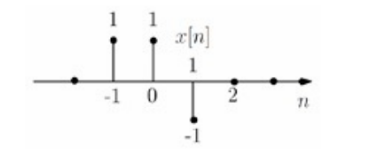
\includegraphics[width=0.5\columnwidth]{figs/q1.png}
    \caption*{}
    \label{fig:placeholder}
\end{figure}


\textbf{Solution}:\\

The Opertation 

\begin{align}
    x\sbrak{n} * x\sbrak{n} = y\sbrak{n} 
\end{align}

Can be written as 

\begin{align}
    \vec{y} = \vec{M}\vec{x}
\end{align}

Where , $\vec{M}$ is a special kind of matrix called a Toeplitz matrix formed from the signal $x\sbrak{n}$

Given , 

\begin{align}
    \vec{x} = \myvec{x\sbrak{-1}\\x\sbrak{0}\\x\sbrak{1}} = \myvec{1\\1\\-1}. \\x\sbrak{n} = 0 , \text{ where } n \notin \cbrak{-1,0,1}
\end{align}

\begin{align}
    \vec{M} = \myvec{x\sbrak{-1}&0&0\\x\sbrak{0}&x\sbrak{-1}&0\\x\sbrak{1}&x\sbrak{0}&x\sbrak{-1}\\0&x\sbrak{1}&x\sbrak{0}\\0&0&x\sbrak{1}}
\end{align}

\begin{align}
    \vec{y} = \vec{M}\myvec{x\sbrak{-1}\\x\sbrak{0}\\x\sbrak{1}} = \myvec{1&0&0\\1&1&0\\-1&1&1\\0&-1&1\\0&0&-1}\myvec{1\\1\\-1}
\end{align}

To find $y\sbrak{-1}$ , we perform matrix multiplication for the second row.

\begin{align}
    y\sbrak{-1} &= \myvec{1&1&0}\myvec{1\\1\\-1}\\
    &=2
\end{align}

Hence, $y\sbrak{-1}= 2$


\end{document}


